\documentclass[11pt,a4paper]{article}

% ─── Packages ────────────────────────────────────────────────────────────────
\usepackage[a4paper, top=2.2cm, bottom=2.2cm, left=2.5cm, right=2.5cm]{geometry}
\usepackage[T1]{fontenc}
\usepackage[utf8]{inputenc}
\usepackage{lmodern}
\usepackage{microtype}
\usepackage{xcolor}
\usepackage{colortbl}
\usepackage{titlesec}
\usepackage{fancyhdr}
\usepackage{graphicx}
\usepackage{booktabs}
\usepackage{tabularx}
\usepackage{array}
\usepackage{longtable}
\usepackage{listings}
\usepackage{enumitem}
\usepackage{tikz}
\usepackage{mdframed}
\usepackage{tcolorbox}
\usepackage{amsmath}
\usepackage{hyperref}
\usepackage{parskip}
\usepackage{setspace}
\usepackage{caption}
\usepackage{float}
\usepackage{pifont}
\usepackage{soul}

\usetikzlibrary{shapes.geometric, arrows.meta, positioning, fit, backgrounds,
                decorations.pathmorphing, shadows, calc}

\tcbuselibrary{breakable, skins}

% ─── Colour Palette ───────────────────────────────────────────────────────────
\definecolor{PrimaryBlue}{HTML}{1A237E}
\definecolor{DeepNavy}{HTML}{0D1B5E}
\definecolor{AccentCyan}{HTML}{00B4D8}
\definecolor{AccentTeal}{HTML}{0096C7}
\definecolor{AccentOrange}{HTML}{F57C00}
\definecolor{AccentGold}{HTML}{FFB300}
\definecolor{LightBg}{HTML}{E8EEF9}
\definecolor{DarkGray}{HTML}{263238}
\definecolor{MidGray}{HTML}{546E7A}
\definecolor{SoftGray}{HTML}{ECEFF1}
\definecolor{RowAlt}{HTML}{F0F4FF}
\definecolor{SuccessGreen}{HTML}{1B5E20}
\definecolor{CodeBg}{HTML}{1E2B3A}
\definecolor{CodeFg}{HTML}{CDD9E5}
\definecolor{RuleLine}{HTML}{1A237E}
\definecolor{MongoGreen}{HTML}{1B5E20}
\definecolor{HiveYellow}{HTML}{E65100}
\definecolor{PigPink}{HTML}{880E4F}
\definecolor{MRBlue}{HTML}{0D47A1}

% ─── Hyperref ─────────────────────────────────────────────────────────────────
\hypersetup{
  colorlinks=true,
  linkcolor=AccentTeal,
  urlcolor=AccentCyan,
  citecolor=AccentOrange,
  pdftitle={Phase 1 Report - Multi-Pipeline ETL Framework},
  pdfauthor={DAS 839 Group}
}

% ─── Section Styling ──────────────────────────────────────────────────────────
\titleformat{\section}{
  \large\bfseries\color{PrimaryBlue}
}{%
  \hspace{-2pt}%
  \tikz[baseline=-0.5ex]\fill[AccentCyan] (0,0) rectangle (4pt,1.1em);%
  \hspace{6pt}%
  \colorbox{PrimaryBlue}{\textcolor{white}{\quad\thesection\quad}}%
}{0.7em}{}[{\color{AccentCyan}\titlerule[1.5pt]}]

\titleformat{\subsection}{
  \normalsize\bfseries\color{DarkGray}
}{%
  \tikz[baseline=-0.4ex]\fill[AccentCyan!60] (0,0) rectangle (3pt,0.9em);%
  \hspace{5pt}\thesubsection%
}{0.6em}{}[{\color{AccentCyan!40}\titlerule[0.6pt]}]

\titleformat{\subsubsection}{
  \normalsize\bfseries\color{MidGray}
}{\thesubsubsection}{0.5em}{}

\titlespacing*{\section}{0pt}{16pt}{7pt}
\titlespacing*{\subsection}{0pt}{12pt}{5pt}
\titlespacing*{\subsubsection}{0pt}{9pt}{3pt}

% ─── Header / Footer ──────────────────────────────────────────────────────────
\pagestyle{fancy}
\fancyhf{}
\fancyhead[L]{\textcolor{AccentCyan}{\small\textbf{DAS 839}}\textcolor{MidGray}{\small\,—\,NoSQL Systems}}
\fancyhead[R]{\textcolor{MidGray}{\small\textit{Phase 1 Report}}\;{\color{AccentCyan}\rule[-1pt]{0.4pt}{9pt}}\;{\textcolor{PrimaryBlue}{\small\bfseries ETL Framework}}}
\fancyfoot[C]{\textcolor{MidGray}{\small---\;\thepage\;---}}
\fancyfoot[L]{\textcolor{AccentCyan!70}{\scriptsize Multi-Pipeline ETL Framework}}
\fancyfoot[R]{\textcolor{MidGray!60}{\scriptsize NASA HTTP Logs}}
\renewcommand{\headrulewidth}{0.6pt}
\renewcommand{\headrule}{\hbox to\headwidth{\color{PrimaryBlue}\leaders\hrule height \headrulewidth\hfill}}
\renewcommand{\footrulewidth}{0.3pt}
\renewcommand{\footrule}{\hbox to\headwidth{\color{AccentCyan!40}\leaders\hrule height \footrulewidth\hfill}}

% ─── Code Listing Style ──────────────────────────────────────────────────────────
\lstdefinestyle{regexstyle}{
  backgroundcolor=\color{CodeBg},
  basicstyle=\ttfamily\small\color{CodeFg},
  breaklines=true,
  frame=l,
  framerule=3pt,
  rulecolor=\color{AccentCyan},
  numbers=none,
  xleftmargin=14pt, xrightmargin=8pt,
  framexleftmargin=10pt,
  aboveskip=8pt, belowskip=8pt,
  tabsize=2,
}

% ─── tcolorbox Environments ─────────────────────────────────────────────────────────
\tcbset{
  basebox/.style={
    breakable, enhanced,
    boxrule=0pt, arc=6pt,
    left=10pt, right=10pt, top=7pt, bottom=7pt,
    fonttitle=\bfseries\small,
    borderline west={3pt}{0pt}{\kvtcb@colframe},
    drop shadow={fill=black!10, opacity=0.35, shadow xshift=1.5pt, shadow yshift=-1.5pt}
  }
}

\newtcolorbox{notebox}[1][]{basebox,
  colback=LightBg, colframe=AccentCyan,
  title={\ding{72}\enspace Note}, #1
}

\newtcolorbox{constraintbox}[1][]{basebox,
  colback=AccentOrange!7, colframe=AccentOrange,
  title={\ding{56}\enspace Implementation Constraint}, #1
}

\newtcolorbox{schematable}[1][]{%
  enhanced, breakable, arc=5pt,
  boxrule=0.5pt, colback=white, colframe=PrimaryBlue!60,
  left=6pt, right=6pt, top=5pt, bottom=5pt, #1
}

\newtcolorbox{mrbox}{basebox,
  colback=MRBlue!7, colframe=MRBlue,
  title={\textbullet\enspace MapReduce Pipeline}, fonttitle=\bfseries\small\color{MRBlue}
}
\newtcolorbox{mongobox}{basebox,
  colback=MongoGreen!7, colframe=MongoGreen,
  title={\textbullet\enspace MongoDB Pipeline}, fonttitle=\bfseries\small\color{MongoGreen}
}
\newtcolorbox{hivebox}{basebox,
  colback=HiveYellow!7, colframe=HiveYellow,
  title={\textbullet\enspace Hive Pipeline}, fonttitle=\bfseries\small\color{HiveYellow}
}
\newtcolorbox{pigbox}{basebox,
  colback=PigPink!7, colframe=PigPink,
  title={\textbullet\enspace Pig Pipeline}, fonttitle=\bfseries\small\color{PigPink}
}

% ─── List styling ─────────────────────────────────────────────────────────────
\setlist[itemize]{leftmargin=*, label={\color{AccentCyan}\small\ding{118}}, itemsep=3pt, topsep=4pt}
\setlist[enumerate]{leftmargin=*, itemsep=3pt, topsep=4pt,
  label={\small\bfseries\color{PrimaryBlue}\arabic*.}}

% ─── Misc ─────────────────────────────────────────────────────────────────────
\setlength{\parskip}{5.5pt}
\captionsetup{font=small, labelfont={bf,color=PrimaryBlue}, labelsep=quad,
  justification=centering, skip=6pt}

% ══════════════════════════════════════════════════════════════════════════════
%  TITLE PAGE
% ══════════════════════════════════════════════════════════════════════════════
\begin{document}

\begin{titlepage}

\begin{tikzpicture}[remember picture, overlay]
  % Full dark background
  \fill[DeepNavy] (current page.south west) rectangle (current page.north east);
  % Large decorative circles
  \fill[AccentCyan, opacity=0.08]
    ([xshift=16cm, yshift=-5cm]current page.north west) circle (7cm);
  \fill[PrimaryBlue!60, opacity=0.25]
    ([xshift=-1cm, yshift=-18cm]current page.north west) circle (6cm);
  \fill[AccentCyan!40, opacity=0.12]
    ([xshift=3cm, yshift=2cm]current page.south west) circle (4.5cm);
  % Top accent stripe (cyan)
  \fill[AccentCyan]
    (current page.north west) rectangle ([yshift=-0.6cm]current page.north east);
  % Bottom bar
  \fill[PrimaryBlue!80]
    (current page.south west) rectangle ([yshift=2.2cm]current page.south east);
  % Thin gold separator above bottom bar
  \fill[AccentGold]
    ([yshift=2.2cm]current page.south west) rectangle ([yshift=2.4cm]current page.south east);
  % White content card
  \node[fill=white, opacity=0.97, rounded corners=10pt,
        minimum width=13cm, minimum height=14cm,
        anchor=center] at ([yshift=0.8cm]current page.center) {};
\end{tikzpicture}

\begin{center}
  \vspace*{0.8cm}
  {\fontsize{10}{13}\selectfont\color{DeepNavy}\textbf{DAS 839 \;\textcolor{AccentCyan}{||}\; NoSQL Systems \;\textcolor{AccentCyan}{||}\; End Semester Project}}

  \vspace{3.0cm}

  % Main title block on white card
  {\fontsize{9}{12}\selectfont\bfseries\color{AccentCyan}\MakeUppercase{Phase 1 Report}}\\[8pt]
  {\fontsize{26}{33}\selectfont\bfseries\color{PrimaryBlue}
    Multi-Pipeline ETL\\[4pt]\& Reporting Framework}\\[10pt]
  {\fontsize{13}{17}\selectfont\color{MidGray}
    for Web Server Log Analytics}

  \vspace{0.7cm}
  {\color{AccentCyan}\rule{9cm}{1.8pt}}
  \vspace{0.6cm}

  \renewcommand{\arraystretch}{1.5}
  \begin{tabular}{r@{\hspace{8pt}:{\hspace{8pt}}}l}
    {\small\color{MidGray}\textit{Course}} &
      {\small\bfseries\color{DarkGray}DAS 839 --- NoSQL Systems}\\[-1pt]
    {\small\color{MidGray}\textit{Date}} &
      {\small\bfseries\color{DarkGray}April 2025}\\[-1pt]
    {\small\color{MidGray}\textit{Group}} &
      {\small\bfseries\color{DarkGray}[Group Number / Members]}\\[-1pt]
    {\small\color{MidGray}\textit{Phase}} &
      {\small\bfseries\color{DarkGray}Phase 1 --- Architecture \& Prototype}\\
  \end{tabular}

  \vspace{1.4cm}
  {\color{SoftGray}\rule{9cm}{0.8pt}}\\[12pt]

  % Backend badges
  {\small\color{MidGray}\textbf{Execution Backends}}\\[8pt]
  \colorbox{MRBlue!15}{\textcolor{MRBlue}{\small\bfseries\;MapReduce\;}}\;\;%
  \colorbox{MongoGreen!15}{\textcolor{MongoGreen}{\small\bfseries\;MongoDB\;}}\;\;%
  \colorbox{HiveYellow!15}{\textcolor{HiveYellow}{\small\bfseries\;Hive\;}}\;\;%
  \colorbox{PigPink!15}{\textcolor{PigPink}{\small\bfseries\;Pig\;}}
\end{center}

\vfill
\begin{tikzpicture}[remember picture, overlay]
  \node[anchor=south, text=white!70, yshift=0.55cm, font=\small\itshape]
    at (current page.south)
    {NASA HTTP Web Server Logs --- Kennedy Space Center (Jul--Aug 1995)};
\end{tikzpicture}
\end{titlepage}

\newpage
\thispagestyle{empty}
\begin{tikzpicture}[remember picture, overlay]
  \fill[PrimaryBlue] (current page.north west) rectangle ([yshift=-1.8cm]current page.north east);
  \fill[AccentCyan] ([yshift=-1.8cm]current page.north west) rectangle ([yshift=-2.0cm]current page.north east);
  \node[anchor=west, text=white, font=\large\bfseries, xshift=2.5cm, yshift=-0.9cm]
    at (current page.north west) {Table of Contents};
  \node[anchor=east, text=AccentCyan!60, font=\small\itshape, xshift=-2.5cm, yshift=-0.9cm]
    at (current page.north east) {DAS 839 --- Multi-Pipeline ETL Framework};
\end{tikzpicture}
\vspace*{2.4cm}
\tableofcontents
\newpage

% ══════════════════════════════════════════════════════════════════════════════
%  SECTION 1 — OVERALL DESIGN
% ══════════════════════════════════════════════════════════════════════════════
\section{Overall Design of the Tool}

\subsection{System Philosophy}

The framework is designed as a \textbf{unified, end-to-end ETL and reporting tool} --- not a collection of independent scripts. A single orchestration layer manages pipeline selection, dataset ingestion, transformation, result storage, and reporting. Swapping the execution backend (MapReduce / MongoDB / Hive / Pig) does not alter any other layer of the system; only the processing engine changes.

\subsection{Component Overview}

The system comprises five tightly coupled components:

\vspace{4pt}
\begin{center}
\renewcommand{\arraystretch}{1.45}
\begin{tabular}{@{} >{}p{3.6cm} p{10.3cm} @{}}
\arrayrulecolor{PrimaryBlue!30}\toprule
\rowcolor{PrimaryBlue} \textcolor{white}{\textbf{Component}} & \textcolor{white}{\textbf{Responsibility}} \\
\midrule
\rowcolor{RowAlt}\textbf{\color{PrimaryBlue}User Interface (UI)} &
  Accepts pipeline selection (one of four systems), dataset path, and batch size. Triggers the ETL engine and passes control to the Reporting Module on completion. \\[2pt]
\textbf{\color{PrimaryBlue}ETL Engine} &
  Orchestrates Extract--Transform--Load. Reads raw logs, invokes the chosen service for parsing and aggregation, and pushes results to the relational database. \\[2pt]
\rowcolor{RowAlt}\textbf{\color{PrimaryBlue}Aggregation Layer} &
  The backend-specific execution layer (MapReduce / MongoDB / Hive / Pig) that computes the three mandatory queries over the structured records. \\[2pt]
\textbf{\color{PrimaryBlue}Relational Database} &
  MySQL or PostgreSQL store holding run metadata and all query results. Acts as the single source of truth for cross-pipeline comparison. \\[2pt]
\rowcolor{RowAlt}\textbf{\color{PrimaryBlue}Reporting Module} &
  Reads the relational database and presents results in structured format. \\
\arrayrulecolor{PrimaryBlue!30}\bottomrule
\end{tabular}
\end{center}

\subsection{System Architecture Diagram}

\begin{figure}[H]
\centering
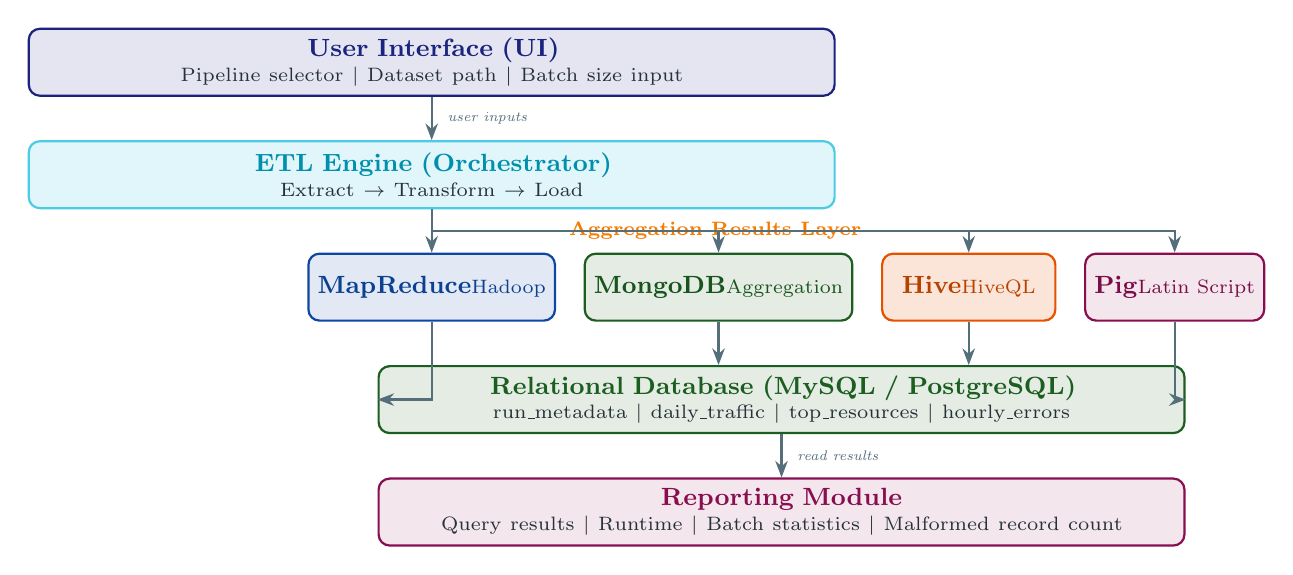
\begin{tikzpicture}[
  node distance = 0.6cm and 0.5cm,
  every node/.style = {font=\small},
  block/.style = {
    rectangle, rounded corners=4pt, minimum width=2.8cm, minimum height=0.85cm,
    text centered, draw, thick
  },
  uiblock/.style   = {block, fill=PrimaryBlue!12, draw=PrimaryBlue, text width=10cm},
  etlblock/.style  = {block, fill=AccentCyan!12, draw=AccentCyan!70, text width=10cm},
  dbblock/.style   = {block, fill=SuccessGreen!12, draw=SuccessGreen, text width=10cm},
  repblock/.style  = {block, fill=PigPink!10, draw=PigPink, text width=10cm},
  arr/.style       = {-{Stealth[length=6pt]}, thick, color=MidGray},
  lbl/.style       = {font=\tiny\itshape, color=MidGray},
]

% UI
\node[uiblock] (ui) {%
  \textbf{\color{PrimaryBlue}User Interface (UI)}\\[-2pt]
  \scriptsize\color{DarkGray} Pipeline selector $|$ Dataset path $|$ Batch size input
};

% ETL
\node[etlblock, below=0.55cm of ui] (etl) {%
  \textbf{\color{AccentCyan!80!black}ETL Engine (Orchestrator)}\\[-2pt]
  \scriptsize\color{DarkGray} Extract $\rightarrow$ Transform $\rightarrow$ Load
};

% Pipeline row
\node[block, fill=MRBlue!12, draw=MRBlue, text=MRBlue!90!black,
      minimum width=2.2cm, below=0.55cm of etl, xshift=0cm] (mr)
      {\textbf{MapReduce}\\[-2pt]\scriptsize Hadoop};
\node[block, fill=MongoGreen!12, draw=MongoGreen, text=MongoGreen!90!black,
      minimum width=2.2cm, right=0.35cm of mr] (mg)
      {\textbf{MongoDB}\\[-2pt]\scriptsize Aggregation};
\node[block, fill=HiveYellow!15, draw=HiveYellow, text=HiveYellow!80!black,
      minimum width=2.2cm, right=0.35cm of mg] (hive)
      {\textbf{Hive}\\[-2pt]\scriptsize HiveQL};
\node[block, fill=PigPink!10, draw=PigPink, text=PigPink!90!black,
      minimum width=2.2cm, right=0.35cm of hive] (pig)
      {\textbf{Pig}\\[-2pt]\scriptsize Latin Script};

% Aggregation label
\node[font=\scriptsize\bfseries\color{AccentOrange},
      above=0.05cm of mr, xshift=3.6cm]
      {Aggregation Results Layer};

% DB
\node[dbblock, below=0.55cm of mg, xshift=0.8cm] (db) {%
  \textbf{\color{SuccessGreen}Relational Database (MySQL / PostgreSQL)}\\[-2pt]
  \scriptsize\color{DarkGray} run\_metadata $|$ daily\_traffic $|$ top\_resources $|$ hourly\_errors
};

% Reporting
\node[repblock, below=0.55cm of db] (rep) {%
  \textbf{\color{PigPink}Reporting Module}\\[-2pt]
  \scriptsize\color{DarkGray} Query results $|$ Runtime $|$ Batch statistics $|$ Malformed record count
};

% Arrows
\draw[arr] (ui) -- (etl) node[lbl, midway, right=2pt] {user inputs};
\draw[arr] (etl.south) -- ++(0,-0.28) -| (mr.north);
\draw[arr] (etl.south) -- ++(0,-0.28) -| (mg.north);
\draw[arr] (etl.south) -- ++(0,-0.28) -| (hive.north);
\draw[arr] (etl.south) -- ++(0,-0.28) -| (pig.north);
\draw[arr] (mr.south) |- (db.west);
\draw[arr] (mg.south) -- (db.north -| mg.south);
\draw[arr] (hive.south) -- (db.north -| hive.south);
\draw[arr] (pig.south) |- (db.east);
\draw[arr] (db) -- (rep) node[lbl, midway, right=2pt] {read results};

\end{tikzpicture}
\caption{System architecture: the unified framework from UI through to the Reporting Module}
\label{fig:arch}
\end{figure}

\subsection{User Interface Design}

The UI is a command-line or lightweight web front-end that presents three inputs to the operator before any computation begins:

\vspace{6pt}
\begin{center}
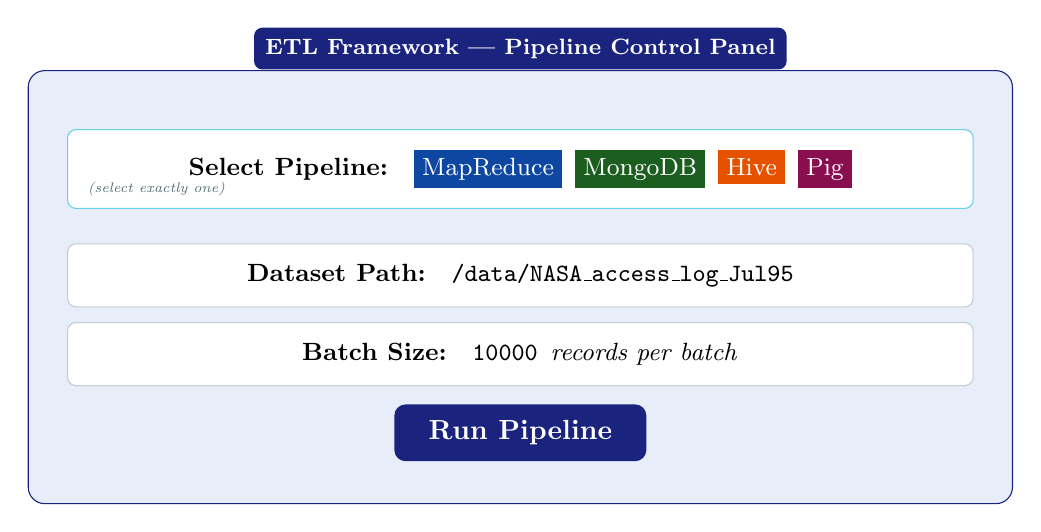
\begin{tikzpicture}[font=\small]
  \node[draw=PrimaryBlue, rounded corners=6pt, fill=LightBg,
        minimum width=12.5cm, minimum height=5.5cm] (panel) {};
  \node[above=0pt of panel.north, anchor=south,
        fill=PrimaryBlue, text=white, rounded corners=3pt,
        inner sep=4pt, font=\bfseries\footnotesize]
    {ETL Framework --- Pipeline Control Panel};

  % Pipeline selector row
  \node[draw=AccentCyan!60, rounded corners=3pt, fill=white, minimum width=11.5cm,
        minimum height=1.0cm, yshift=1.5cm] (ps) {%
    \textbf{Select Pipeline:}\quad
    \colorbox{MRBlue}{\textcolor{white}{\small MapReduce}}\enspace
    \colorbox{MongoGreen}{\textcolor{white}{\small MongoDB}}\enspace
    \colorbox{HiveYellow}{\textcolor{white}{\small Hive}}\enspace
    \colorbox{PigPink}{\textcolor{white}{\small Pig}}%
  };
  \node[font=\tiny\itshape\color{MidGray}, above=1pt of ps.south west, anchor=south west,
        xshift=4pt]{(select exactly one)};

  % Dataset path row
  \node[draw=MidGray!35, rounded corners=3pt, fill=white, minimum width=11.5cm,
        minimum height=0.8cm, yshift=0.15cm]
    {\textbf{Dataset Path:}\quad\texttt{/data/NASA\_access\_log\_Jul95}};

  % Batch size row
  \node[draw=MidGray!35, rounded corners=3pt, fill=white, minimum width=11.5cm,
        minimum height=0.8cm, yshift=-0.85cm]
    {\textbf{Batch Size:}\quad\texttt{10000}\enspace\textit{\small records per batch}};

  % Run button
  \node[fill=PrimaryBlue, text=white, rounded corners=4pt,
        minimum width=3.2cm, minimum height=0.72cm, yshift=-1.85cm,
        font=\bfseries]
    {Run Pipeline};
\end{tikzpicture}
\end{center}

\vspace{4pt}
After execution, the UI passes control to the Reporting Module, which reads the relational database and renders structured results including query output tables, wall-clock runtime, batch statistics, and the malformed-record count.

\subsection{Reporting Module}

The Reporting Module reads from the relational database and presents:
\begin{itemize}
  \item \textbf{Run metadata:} pipeline name, run ID, batch ID, batch size, total runtime (seconds), malformed count
  \item \textbf{Query 1 table} --- Daily Traffic Summary (grouped by date and status code)
  \item \textbf{Query 2 table} --- Top 20 Requested Resources
  \item \textbf{Query 3 table} --- Hourly Error Analysis (grouped by date and hour)
\end{itemize}

\begin{notebox}
The framework is a single coherent tool. The execution backend is a pluggable module; all other components (UI, orchestration, database schema, reporting) remain identical across all four pipelines.
\end{notebox}

% ══════════════════════════════════════════════════════════════════════════════
%  SECTION 2 — PARSING STRATEGY
% ══════════════════════════════════════════════════════════════════════════════
\section{Parsing Strategy}
\label{sec:parsing}

\subsection{Log Format}

Each line in the NASA HTTP log follows the Combined Log Format. A representative record is:

\begin{tcolorbox}[basebox, colback=DarkGray!90, colframe=DarkGray,
                  fontupper=\ttfamily\small\color{white}]
199.72.81.55 - - [01/Jul/1995:00:00:01 -0400] "GET /history/apollo/ HTTP/1.0" 200 6245
\end{tcolorbox}

\subsection{Extracted Fields}

\vspace{4pt}
\begin{center}
\renewcommand{\arraystretch}{1.35}
\begin{tabular}{@{} >{\ttfamily\small}l >{\small}l >{\small\itshape}l @{}}
\toprule
\textnormal{\textbf{Raw value}} & \textbf{Extracted field} & \textbf{Notes} \\
\midrule
199.72.81.55              & host             & IP address or hostname \\
01/Jul/1995:00:00:01 -0400 & timestamp        & Full timestamp string \\
01/Jul/1995               & log\_date        & Date portion extracted from timestamp \\
00                        & log\_hour        & Hour portion (0--23) \\
GET                       & http\_method     & First token of the quoted request \\
/history/apollo/          & resource\_path   & Second token \\
HTTP/1.0                  & protocol\_version & Third token \\
200                       & status\_code     & Integer HTTP reply code \\
6245                      & bytes\_transferred & Integer; \texttt{-} is treated as 0 \\
\bottomrule
\end{tabular}
\end{center}

\subsection{Regex-Based Parsing}

A single master regular expression captures all top-level fields in one pass. Sub-fields of the request string (method, path, protocol) and the timestamp (date, hour) are extracted from the captured groups:

\begin{lstlisting}[style=regexstyle, caption={Master regular expression for log-line parsing}]
^(\S+)\s+\S+\s+\S+\s+
\[(\d{2}/\w{3}/\d{4}):(\d{2}):\d{2}:\d{2}\s+[+-]\d{4}\]\s+
"([A-Z]+)\s+(\S+)\s+(HTTP/[\d.]+)"\s+
(\d{3})\s+(\S+)$
\end{lstlisting}

Capture-group mapping:
\texttt{(1)~host}, \texttt{(2)~log\_date}, \texttt{(3)~log\_hour}, \texttt{(4)~http\_method},
\texttt{(5)~resource\_path}, \texttt{(6)~protocol\_version}, \texttt{(7)~status\_code},
\texttt{(8)~bytes\_raw}.

The \texttt{bytes\_transferred} field is derived as:
\[
  \text{bytes\_transferred} =
  \begin{cases}
    0 & \text{if } \texttt{bytes\_raw} = \texttt{"-"} \\
    \text{int}(\texttt{bytes\_raw}) & \text{otherwise}
  \end{cases}
\]

\subsection{Parsing Constraints}

\begin{constraintbox}
\begin{itemize}
  \item If the bytes field contains \texttt{-}, it \textbf{must} be substituted with \textbf{0} (not discarded).
  \item Malformed records (lines that do not match the master regex) must \textbf{not} be silently dropped. A \texttt{malformed\_record\_counter} is incremented and the count is persisted to the metadata table at the end of each run.
  \item Dataset path and batch size are \textbf{user inputs} supplied via the UI; they are not hardcoded anywhere in the codebase.
\end{itemize}
\end{constraintbox}

\subsection{Parsing Flow Diagram}

\begin{figure}[H]
\centering
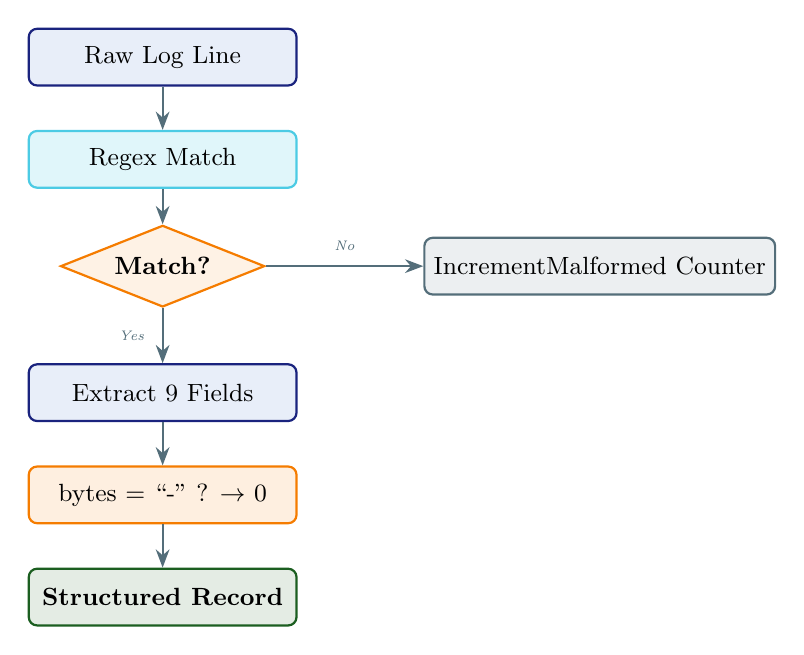
\begin{tikzpicture}[
  node distance=0.55cm,
  box/.style={rectangle, rounded corners=3pt, draw, thick, minimum width=3.4cm,
              minimum height=0.72cm, text centered, font=\small},
  decision/.style={diamond, draw=AccentOrange, thick, fill=AccentOrange!10,
                   aspect=2.5, minimum height=0.8cm,
                   text centered, font=\small\bfseries},
  arr/.style={-{Stealth}, thick, MidGray},
  lbl/.style={font=\tiny\itshape, MidGray},
]

\node[box, fill=LightBg, draw=PrimaryBlue] (raw) {Raw Log Line};
\node[box, fill=AccentCyan!12, draw=AccentCyan!70, below=of raw] (regex) {Regex Match};
\node[decision, below=0.45cm of regex] (match) {Match?};
\node[box, fill=SoftGray, draw=MidGray, right=2cm of match] (bad)
  {Increment\\Malformed Counter};
\node[box, fill=LightBg, draw=PrimaryBlue, below=0.7cm of match] (fields)
  {Extract 9 Fields};
\node[box, fill=AccentOrange!12, draw=AccentOrange, below=of fields] (bytes)
  {bytes = ``-'' ? $\to$ 0};
\node[box, fill=SuccessGreen!12, draw=SuccessGreen, below=of bytes] (struct)
  {\textbf{Structured Record}};

\draw[arr] (raw) -- (regex);
\draw[arr] (regex) -- (match);
\draw[arr] (match) -- node[lbl, left=3pt]{Yes} (fields);
\draw[arr] (match) -- node[lbl, above=2pt]{No} (bad);
\draw[arr] (fields) -- (bytes);
\draw[arr] (bytes) -- (struct);

\end{tikzpicture}
\caption{Parsing flow: from raw log line to validated structured record}
\label{fig:parse}
\end{figure}

% ══════════════════════════════════════════════════════════════════════════════
%  SECTION 3 — ETL WORKFLOW
% ══════════════════════════════════════════════════════════════════════════════
\section{ETL Workflow}

The ETL workflow is \textbf{logically identical} across all four pipelines. Only the execution engine differs.

\subsection{Three Phases}

\subsubsection{Extract}
Raw log files are read from the path supplied by the user through the UI. No preprocessing outside the chosen execution pipeline is permitted (no manual CSV conversion, JSON conversion, filtering, or editing). Files are read line by line and dispatched to the transform stage in configurable batches.

\subsubsection{Transform}
\begin{itemize}
  \item \textbf{Parsing} --- the master regex is applied to each record (see Section~\ref{sec:parsing}).
  \item \textbf{Cleaning} --- \texttt{-} bytes are substituted with \texttt{0}; malformed lines increment the counter.
  \item \textbf{Field extraction} --- each valid record is promoted to a typed, structured representation carrying all nine fields.
\end{itemize}

\subsubsection{Load}
\begin{itemize}
  \item The three mandatory queries are executed on the structured data within the chosen backend.
  \item Aggregated results are written to the relational database (MySQL or PostgreSQL).
  \item Run metadata (runtime, malformed count, batch statistics) is inserted into the \texttt{run\_metadata} table.
\end{itemize}

\subsection{ETL Flow Diagram}

\begin{figure}[H]
\centering
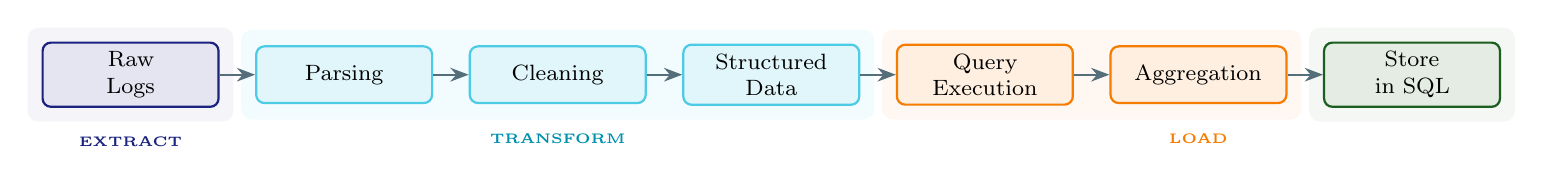
\begin{tikzpicture}[
  node distance = 0.4cm,
  stage/.style = {rectangle, rounded corners=3pt, draw, thick,
                  minimum width=2.2cm, minimum height=0.72cm,
                  text centered, font=\footnotesize, text width=2.0cm},
  arr/.style = {-{Stealth}, thick, MidGray},
]

\node[stage, fill=PrimaryBlue!12, draw=PrimaryBlue]   (raw)    {Raw\\Logs};
\node[stage, fill=AccentCyan!12, draw=AccentCyan!70,
      right=0.45cm of raw]                            (parse)  {Parsing};
\node[stage, fill=AccentCyan!12, draw=AccentCyan!70,
      right=0.45cm of parse]                          (clean)  {Cleaning};
\node[stage, fill=AccentCyan!12, draw=AccentCyan!70,
      right=0.45cm of clean]                          (struct) {Structured\\Data};
\node[stage, fill=AccentOrange!12, draw=AccentOrange,
      right=0.45cm of struct]                         (query)  {Query\\Execution};
\node[stage, fill=AccentOrange!12, draw=AccentOrange,
      right=0.45cm of query]                          (agg)    {Aggregation};
\node[stage, fill=SuccessGreen!12, draw=SuccessGreen,
      right=0.45cm of agg]                            (db)     {Store\\in SQL};

\draw[arr] (raw)--(parse);
\draw[arr] (parse)--(clean);
\draw[arr] (clean)--(struct);
\draw[arr] (struct)--(query);
\draw[arr] (query)--(agg);
\draw[arr] (agg)--(db);

% Phase labels below
\node[font=\tiny\bfseries\color{PrimaryBlue},
      below=0.25cm of raw] {EXTRACT};
\node[font=\tiny\bfseries\color{AccentCyan!80!black},
      below=0.25cm of clean] {TRANSFORM};
\node[font=\tiny\bfseries\color{AccentOrange},
      below=0.25cm of agg] {LOAD};

% Background shading
\begin{scope}[on background layer]
  \node[fill=PrimaryBlue!5, rounded corners=4pt,
        fit=(raw), inner sep=5pt] {};
  \node[fill=AccentCyan!5, rounded corners=4pt,
        fit=(parse)(clean)(struct), inner sep=5pt] {};
  \node[fill=AccentOrange!5, rounded corners=4pt,
        fit=(query)(agg), inner sep=5pt] {};
  \node[fill=SuccessGreen!5, rounded corners=4pt,
        fit=(db), inner sep=5pt] {};
\end{scope}

\end{tikzpicture}
\caption{ETL workflow -- common across all four pipelines}
\label{fig:etl}
\end{figure}

\begin{notebox}
The parsing rules, cleaning rules, field definitions, query definitions, and output schema are strictly identical across MapReduce, MongoDB, Hive, and Pig. This ensures cross-pipeline comparisons are fair and meaningful.
\end{notebox}

% ══════════════════════════════════════════════════════════════════════════════
%  SECTION 4 — PIPELINE OVERVIEW
% ══════════════════════════════════════════════════════════════════════════════
\section{Pipeline Overview}

Each pipeline executes the same three analytical queries using a different processing paradigm. All four implement equivalent semantics: the same parsing rules, cleaning rules, filtering conditions, grouping logic, and aggregation definitions.

\begin{mrbox}
\textbf{Paradigm:} Low-level, programmer-controlled parallel computation on HDFS.

\textbf{Execution model:} Custom Mapper and Reducer classes. The Mapper applies the master regex to each log line and emits typed key--value pairs. The Reducer aggregates values per key (e.g., summing bytes, counting requests, collecting distinct hosts).

\textbf{Characteristics:} Fine-grained control over the map phase, shuffle/sort, and reduce phase. Hadoop's \texttt{InputSplit} mechanism naturally partitions data into processing chunks that correspond to logical batches.

\textbf{Query implementation:} Each of the three queries is a separate MapReduce job. Jobs are chained by the orchestrator, and results are loaded to SQL at the end of each chain.
\end{mrbox}

\vspace{5pt}

\begin{mongobox}
\textbf{Paradigm:} Document-oriented NoSQL with a declarative aggregation framework.

\textbf{Execution model:} Parsed log records are inserted as BSON documents into a collection. Queries are expressed using the MongoDB Aggregation Pipeline: \texttt{\$match} for filtering, \texttt{\$group} for aggregation, \texttt{\$sort} and \texttt{\$limit} for top-$N$ ranking.

\textbf{Characteristics:} Schema-flexible; easy to express the three queries in a concise, declarative style. Data is inserted in configurable-size chunks (batches) tracked by batch ID.
\end{mongobox}

\vspace{5pt}

\begin{hivebox}
\textbf{Paradigm:} SQL-like query language (HiveQL) over Hadoop.

\textbf{Execution model:} The log file is loaded into an external Hive table backed by the raw text. Queries are written as standard \texttt{SELECT ... GROUP BY ...} HiveQL statements. Hive compiles these internally into MapReduce or Tez jobs.

\textbf{Characteristics:} The three mandatory queries map almost directly to SQL, making Hive the most concise implementation. Partitioning or chunk-based loading is used to emulate batching.
\end{hivebox}

\vspace{5pt}

\begin{pigbox}
\textbf{Paradigm:} Dataflow scripting language (Pig Latin) that compiles to MapReduce.

\textbf{Execution model:} A Pig Latin script loads the data, applies a custom UDF or regex-based \texttt{LOAD} function for parsing, then uses \texttt{FILTER}, \texttt{GROUP}, and \texttt{FOREACH ... GENERATE} to compute the required aggregations.

\textbf{Characteristics:} Step-by-step, explicit transformation pipeline. Each data transformation is visible as a named Pig relation, making the logic easy to audit and debug.
\end{pigbox}

% ══════════════════════════════════════════════════════════════════════════════
%  SECTION 5 — BATCHING APPROACH
% ══════════════════════════════════════════════════════════════════════════════
\section{Batching Approach}

\subsection{Definition}

\begin{tcolorbox}[basebox, colback=LightBg, colframe=AccentCyan,
                  title={Batch Definition}]
\textbf{Batch} = a fixed number of input log records processed together in one execution unit.

\begin{itemize}
  \item \textbf{Batch size} --- configurable integer supplied by the user via the UI (e.g.\ 10\,000 records).
  \item \textbf{Batch ID} --- sequential integer starting from \textbf{1}, incrementing by 1 for each subsequent batch.
  \item \textbf{Final batch} --- if the last group contains fewer records than the configured batch size, it is still counted as a valid batch and given the next sequential ID.
\end{itemize}
\end{tcolorbox}

The \textbf{average batch size} is reported as:
\[
  \overline{\text{batch size}} \;=\;
  \frac{\text{total records processed}}{\text{number of non-empty batches}}
\]

\subsection{Pipeline-Specific Batching}

\begin{center}
\renewcommand{\arraystretch}{1.4}
\begin{tabularx}{\linewidth}{@{} >{\bfseries\small}l X @{}}
\toprule
Pipeline & Batching mechanism \\
\midrule
MapReduce &
  Hadoop's \texttt{NLineInputFormat} is configured so that each InputSplit contains exactly \emph{N} lines, where \emph{N} equals the chosen batch size. Each InputSplit is processed by one Mapper, constituting one logical batch. \\[3pt]
MongoDB &
  Parsed records are inserted via \texttt{insert\_many()} in Python list chunks of size $= $ batch size. Each \texttt{insert\_many()} call represents one batch; \texttt{batch\_id} is tracked and stored per chunk in the metadata table. \\[3pt]
Hive &
  The orchestrator splits the raw log file into chunk files, each containing exactly \emph{batch\_size} lines. Chunk files are loaded sequentially into the Hive table, and each load operation is assigned a sequential \texttt{batch\_id}. \\[3pt]
Pig &
  Pre-split chunk files (produced by the orchestrator) are passed to Pig runs sequentially. Each Pig execution processes one chunk, corresponding to one batch. \\
\bottomrule
\end{tabularx}
\end{center}

\subsection{Batch Processing Diagram}

\begin{figure}[H]
\centering
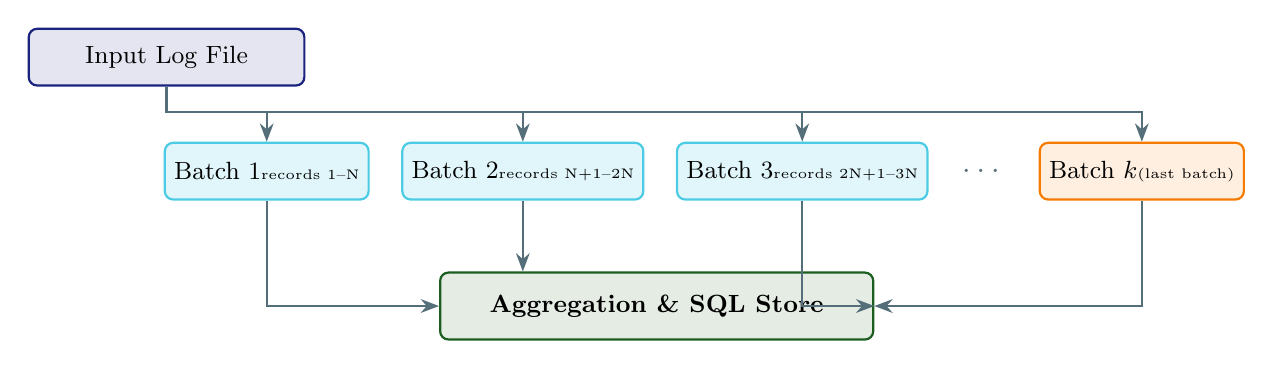
\begin{tikzpicture}[
  node distance=0.5cm and 0.5cm,
  box/.style={rectangle, rounded corners=3pt, draw, thick,
              minimum width=2.3cm, minimum height=0.72cm,
              text centered, font=\small},
  arr/.style={-{Stealth}, thick, MidGray},
]

\node[box, fill=PrimaryBlue!12, draw=PrimaryBlue, minimum width=3.5cm] (input)
  {Input Log File};

\node[box, fill=AccentCyan!12, draw=AccentCyan!70,
      below right=0.7cm and -1.8cm of input] (b1)
  {Batch 1\\{\tiny records 1--N}};
\node[box, fill=AccentCyan!12, draw=AccentCyan!70,
      right=0.4cm of b1] (b2)
  {Batch 2\\{\tiny records N+1--2N}};
\node[box, fill=AccentCyan!12, draw=AccentCyan!70,
      right=0.4cm of b2] (b3)
  {Batch 3\\{\tiny records 2N+1--3N}};
\node[font=\large\color{MidGray}, right=0.3cm of b3] (dots) {\ldots};
\node[box, fill=AccentOrange!12, draw=AccentOrange,
      right=0.3cm of dots] (bn)
  {Batch $k$\\{\tiny (last batch)}};

\node[box, fill=SuccessGreen!12, draw=SuccessGreen,
      below=0.9cm of b2, xshift=1.7cm, minimum width=5.5cm,
      minimum height=0.85cm] (agg)
  {\textbf{Aggregation \& SQL Store}};

\draw[arr] (input.south) -- ++(0,-0.32) -| (b1.north);
\draw[arr] (input.south) -- ++(0,-0.32) -| (b2.north);
\draw[arr] (input.south) -- ++(0,-0.32) -| (b3.north);
\draw[arr] (input.south) -- ++(0,-0.32) -| (bn.north);

\draw[arr] (b1.south) |- (agg.west);
\draw[arr] (b2.south) -- (agg.north -| b2.south);
\draw[arr] (b3.south) |- (agg);
\draw[arr] (bn.south) |- (agg.east);

\end{tikzpicture}
\caption{Batch processing: input is partitioned into $k$ equal batches; the final batch may contain fewer than $N$ records}
\label{fig:batch}
\end{figure}

% ══════════════════════════════════════════════════════════════════════════════
%  SECTION 6 — RELATIONAL DATABASE SCHEMA
% ══════════════════════════════════════════════════════════════════════════════
\section{Relational Database Schema}

\subsection{Design Rationale}

The schema separates run-level metadata from query results. One metadata table stores information common to all queries (pipeline name, runtime, batch info). Three result tables---one per mandatory query---hold the aggregated outputs and reference the metadata table via \texttt{run\_id} (foreign key). This design allows any run's results to be retrieved, filtered by pipeline or batch, and compared against other runs.

\subsection{Metadata Table: \texttt{run\_metadata}}

\begin{schematable}
\begin{tabularx}{\linewidth}{@{} >{\ttfamily\small}l >{\small}l X @{}}
\toprule
\textnormal{\textbf{Column}} & \textbf{Type} & \textbf{Description} \\
\midrule
run\_id              & SERIAL PK    & Auto-incremented unique identifier for each run \\
pipeline\_name       & VARCHAR(20)  & One of: \texttt{mapreduce}, \texttt{mongodb}, \texttt{hive}, \texttt{pig} \\
batch\_id            & INTEGER      & Sequential batch identifier (starts at 1) \\
batch\_size          & INTEGER      & Configured number of records per batch \\
avg\_batch\_size      & FLOAT        & Actual average records across all batches processed \\
runtime              & FLOAT        & Wall-clock time in seconds (ETL only; excludes report time) \\
malformed\_record\_count & INTEGER  & Number of log lines that failed regex parsing \\
timestamp            & TIMESTAMP    & UTC datetime when the run was recorded \\
\bottomrule
\end{tabularx}
\end{schematable}

\subsection{Result Table 1: \texttt{daily\_traffic}}

Stores the output of Query 1 (Daily Traffic Summary).

\begin{schematable}
\begin{tabularx}{\linewidth}{@{} >{\ttfamily\small}l >{\small}l X @{}}
\toprule
\textnormal{\textbf{Column}} & \textbf{Type} & \textbf{Description} \\
\midrule
id            & SERIAL PK  & Row identifier \\
run\_id       & INTEGER FK & References \texttt{run\_metadata.run\_id} \\
log\_date     & DATE       & Date of the log entries (e.g.\ 01/Jul/1995) \\
status\_code  & INTEGER    & HTTP reply code \\
request\_count & BIGINT    & Total number of requests for this date--code pair \\
total\_bytes  & BIGINT     & Sum of bytes transferred for this date--code pair \\
\bottomrule
\end{tabularx}
\end{schematable}

\subsection{Result Table 2: \texttt{top\_resources}}

Stores the output of Query 2 (Top Requested Resources). Only the top 20 rows by request count are stored per run.

\begin{schematable}
\begin{tabularx}{\linewidth}{@{} >{\ttfamily\small}l >{\small}l X @{}}
\toprule
\textnormal{\textbf{Column}} & \textbf{Type} & \textbf{Description} \\
\midrule
id                 & SERIAL PK  & Row identifier \\
run\_id            & INTEGER FK & References \texttt{run\_metadata.run\_id} \\
resource\_path     & TEXT       & Requested URL path \\
request\_count     & BIGINT     & Number of times this resource was requested \\
total\_bytes       & BIGINT     & Total bytes served for this resource \\
distinct\_host\_count & BIGINT  & Number of unique hosts requesting this resource \\
\bottomrule
\end{tabularx}
\end{schematable}

\subsection{Result Table 3: \texttt{hourly\_errors}}

Stores the output of Query 3 (Hourly Error Analysis).

\begin{schematable}
\begin{tabularx}{\linewidth}{@{} >{\ttfamily\small}l >{\small}l X @{}}
\toprule
\textnormal{\textbf{Column}} & \textbf{Type} & \textbf{Description} \\
\midrule
id                    & SERIAL PK  & Row identifier \\
run\_id               & INTEGER FK & References \texttt{run\_metadata.run\_id} \\
log\_date             & DATE       & Date of the log entries \\
log\_hour             & SMALLINT   & Hour of day (0--23) \\
error\_request\_count  & BIGINT     & Requests with status code 400--599 \\
total\_request\_count  & BIGINT     & All requests in this date--hour slot \\
error\_rate           & FLOAT      & \texttt{error\_request\_count / total\_request\_count} \\
distinct\_error\_hosts & BIGINT     & Unique hosts generating error responses \\
\bottomrule
\end{tabularx}
\end{schematable}

% ══════════════════════════════════════════════════════════════════════════════
%  SECTION 7 — EQUIVALENCE ACROSS PIPELINES
% ══════════════════════════════════════════════════════════════════════════════
\section{Ensuring Equivalence Across Pipelines}

To make the cross-pipeline comparison fair and meaningful, the following invariants are enforced throughout the implementation:

\begin{enumerate}
  \item \textbf{Same dataset.} All pipelines read the identical NASA HTTP log files downloaded from the official Internet Traffic Archive. No manual preprocessing, CSV conversion, JSON conversion, filtering, or editing is applied outside the selected pipeline.

  \item \textbf{Same parsing rules.} The master regex and field-extraction logic are defined once at the architecture level and translated faithfully into each backend (Mapper code, MongoDB UDF, Hive SerDe or regex UDF, Pig LOAD function with UDF).

  \item \textbf{Same query definitions.} The three mandatory queries specify exact output columns, filtering conditions (e.g.\ status 400--599 for errors), and aggregation semantics. These are not relaxed or simplified for any particular pipeline.

  \item \textbf{Same batch size.} In any comparative experiment, the same batch-size value is supplied to all four pipelines via the shared UI.

  \item \textbf{Same output schema.} All results are written to the shared relational database in an identical schema regardless of which backend produced them. This allows direct SQL comparison across runs.
\end{enumerate}

% ══════════════════════════════════════════════════════════════════════════════
%  SECTION 8 — DIAGRAM INDEX
% ══════════════════════════════════════════════════════════════════════════════
\section{Diagram Index}

\begin{center}
\renewcommand{\arraystretch}{1.45}
\begin{tabular}{@{} c >{\bfseries}l l @{}}
\arrayrulecolor{PrimaryBlue!30}\toprule
\rowcolor{PrimaryBlue}
  \textcolor{white}{\textbf{Figure}} & \textcolor{white}{\textbf{Section}} & \textcolor{white}{\textbf{Description}} \\
\midrule
\rowcolor{RowAlt}\ref{fig:arch}  & 1 & System Architecture --- UI through to Reporting Module \\
\ref{fig:parse} & 2 & Parsing Flow --- Raw line to validated structured record \\
\rowcolor{RowAlt}\ref{fig:etl}   & 3 & ETL Workflow --- Extract, Transform, Load \\
\ref{fig:batch} & 5 & Batch Processing --- Input split into $k$ equal batches \\
\arrayrulecolor{PrimaryBlue!30}\bottomrule
\end{tabular}
\end{center}

% ══════════════════════════════════════════════════════════════════════════════
%  SECTION 9 — PHASE 1 STATUS
% ══════════════════════════════════════════════════════════════════════════════
\section{Phase 1 Prototype Status}

At the time of this Phase 1 review, the following components are complete or in active development:

\begin{center}
\renewcommand{\arraystretch}{1.4}
\begin{tabular}{@{} l c c @{}}
\arrayrulecolor{PrimaryBlue!30}\toprule
\rowcolor{PrimaryBlue}
  \textcolor{white}{\textbf{Component}} & \textcolor{white}{\textbf{Status}} & \textcolor{white}{\textbf{Applies to}} \\
\midrule
\rowcolor{SuccessGreen!8}UI (pipeline selector, dataset path, batch size) & \textcolor{SuccessGreen}{\ding{52}\;Done} & All \\
\rowcolor{SuccessGreen!8}Master regex parser + malformed counter           & \textcolor{SuccessGreen}{\ding{52}\;Done} & All \\
\rowcolor{SuccessGreen!8}MapReduce ETL (Q1, Q2, Q3)                        & \textcolor{SuccessGreen}{\ding{52}\;Done} & MapReduce \\
\rowcolor{SuccessGreen!8}MongoDB ETL (Q1, Q2, Q3)                          & \textcolor{SuccessGreen}{\ding{52}\;Done} & MongoDB \\
\rowcolor{AccentOrange!10}Hive ETL                                          & \textcolor{AccentOrange}{\ding{115}\;In Progress} & Hive \\
\rowcolor{AccentOrange!10}Pig ETL                                           & \textcolor{AccentOrange}{\ding{115}\;In Progress} & Pig \\
\rowcolor{SuccessGreen!8}Relational database schema and load scripts        & \textcolor{SuccessGreen}{\ding{52}\;Done} & All \\
\rowcolor{SuccessGreen!8}Reporting module                                   & \textcolor{SuccessGreen}{\ding{52}\;Done} & All \\
\arrayrulecolor{PrimaryBlue!30}\bottomrule
\end{tabular}
\end{center}

Phase 2 will complete the Hive and Pig pipelines, execute comparative experiments across all four backends using the same batch size, and document runtime observations, implementation difficulty, and correctness comparisons.

\vspace{1.5cm}
\begin{center}
\begin{tcolorbox}[enhanced, arc=8pt, boxrule=0pt,
  colback=PrimaryBlue, colframe=PrimaryBlue,
  width=10cm, halign=center,
  drop shadow={fill=black!20, opacity=0.4}]
  \centering
  {\color{AccentCyan}\rule{6cm}{0.6pt}}\\[6pt]
  {\small\color{white}\itshape End of Phase 1 Report}\\[3pt]
  {\small\color{AccentCyan!80}\bfseries DAS 839 \;\textcolor{white}{||}\; NoSQL Systems}\\[6pt]
  {\color{AccentCyan}\rule{6cm}{0.6pt}}
\end{tcolorbox}
\end{center}

\end{document}